\chapter{実験1 : MNISTを用いた予備実験}

\section{概要}
本章では、本研究で提案するQuery-By-Dropout-Predictionsの有効性を検証するためにMNISTに対して行った実験について説明する。
Dropoutによってサンプリングされた各部分ネットワークの出力が未知データに対して分散を持つのかを検証し、
能動学習のクエリ選考基準として有効であるかを確認する。


\section{実験設定}

\subsection{データセットについて}
MNISTは28×28ピクセルの手書き数字のデータセットである。
7万枚の画像からなり、そのうちの6万枚は訓練画像、残りの1万枚はテスト画像として利用される。
それぞれの画像は0~9までの数字ラベルが割り当てられているが、能動学習の状況を再現するため、
クエリとして問い合わせられるまではラベルへのアクセスが与えられない状況を設定する。


\subsection{実験の詳細}

\begin{table}[h]
    \label{table:mnist_cnn}
    \caption{MNISTの実験に使用したCNNの構造を示す。}
    \center
    \begin{tabular}{|c|c|c|} \hline
        layer & size & activation \\ \hline
        Convolution & $32 \times 4 \times 4$ & relu \\
        Convolution & $32 \times 4 \times 4$ & relu \\
        Max Pooling & & \\
        dropout & & \\
        fully connected & 128 & relu \\
        dropout & & \\
        fully connected & 128 & relu \\
        \hline
    \end{tabular}
  \end{table}

識別器にはCNNを利用する。その構造を以下に示す\ref{table:mnist_cnn}(Kerasのexampleプログラムを参考にした)。
比較的小さなCNNであるため、クエリ問い合わせによってラベルが追加されるごとにfrom scratchからの再学習を行うことにする。
多層ニューラルネットワークの中では小さいモデルではあるものの、ラベルを一つずつ追加して再学習を行うのは計算コストが大きいため、バッチ型能動学習を採用する。
ここでも、同一クエリ内での情報の重複を避けるためクラスタリングを行う。
MNISTは784次元の画像で比較的小さいため、元の画像情報をそのまま特徴量としてk-meansによるクラスタリングを行う。
committeeサイズは10, k-meansのクラスター数$K$は100、一度に選択するクエリ$\mathcal{Q}$のサイズは10、再学習のepoch数は100に設定した。
また、クラスターの代表サンプルから無作為にサンプリングされた20個のサンプルをラベルを付与して学習初期のラベルつきデータとして実験を開始した。
訓練時にはcrop領域をランダムにずらすAugmentationを利用した。
各クエリ問い合わせ毎に10000枚のテストデータに対する識別精度を計測し、ラベルを付与されたデータが1000に到達するまで実験を続けた。
実験ごとのばらつきを考慮し、同一の実験を3回行いその平均と標準偏差を計算した。

\subsection{比較手法について}
提案するQuery-By-Dropout-Predictionsの性能を比較するため、いくつかの手法について実験を行った。
クエリの選考基準以外は全ての設定を揃えて実験を行った。

\subsubsection{Random Sampling}
この実験のベースラインと言える選択基準。各クエリ問い合わせ毎にランダムにサンプルを選択してラベル付きデータセットに追加する。

\subsubsection{Uncertainty Sampling}
推論時にDropoutを使用せずに単一の予測分布のエントロピーを利用する。
\begin{eqnarray}
    score(x) =  - \sum_i {P_{\theta}(y_i|x)} \log P_{\theta}(y|x)
\end{eqnarray}

\subsubsection{Query-By-Dropout-Predictions $+$ Uncertain Sampling}
推論時にDropoutを利用し、複数のpredictionを出力しそれらの平均の不確かさと不一致度を基準として利用する。
不確かさには予測分布のエントロピー(Entropy Sampling)を利用する。
\begin{eqnarray}
    score(x) =  -  \frac{1}{C} \sum_{c=i}^C KL \, (P_{\theta^{(c)}} || P_C) \, - \sum_i {P_C(y_i|x)} \log P_C(y|x)
\end{eqnarray}

\subsubsection{Query-By-Dropout-Predictions $+$ Uncertain Sampling $+$ 推論時Data Augmentation}
上記のクエリ基準に加え、推論時にもData Augmentationを利用することで特徴抽出層の学習に有効だと考えられるサンプルも選択できるようにする。
% \subsubsection{Dropoutにより周辺化した予測分布を利用したUncertainty Sampling}
% 推論時にDropoutを使用せずに単一の予測分布のエントロピーを利用する。\todo{このへんあやしいベイズCNNの話しないと}
% \begin{eqnarray}
%     score(x) =  - \sum_i {P_C(y_i|x)} \log P_C(y|x)
% \end{eqnarray}

\section{実験結果}
本項では上記で述べた実験の結果を示す。
クエリ選考基準として提案手法、比較手法それぞれを使用した際の、ラベル付きサンプル数の増加に対するテスト精度の変化のグラフを図\ref{fig:mnist_acc_graph}に示す。
また、テストデータの識別精度が$90\%$、$95\%$、 $98\%$を超えるのに要したラベルの数を表\ref{table:mnist_samplenum_accuracy}に示す。
提案したQuery-By-Dropout-Committeeの手法がUncertain Samplingのみを使用した場合と比較して性能が良いことがわかる。
これは上記に述べた通り多層ニューラルネットワークが正しくモデルの不確かさを表現できていないからだと推測される。
さらに、推論時にもData Augmentationを利用することで、さらに少ないラベルで高精度を達成していることがわかる。

\begin{figure}[tbp]
    \label{fig:mnist_acc_graph}
     \begin{center}
      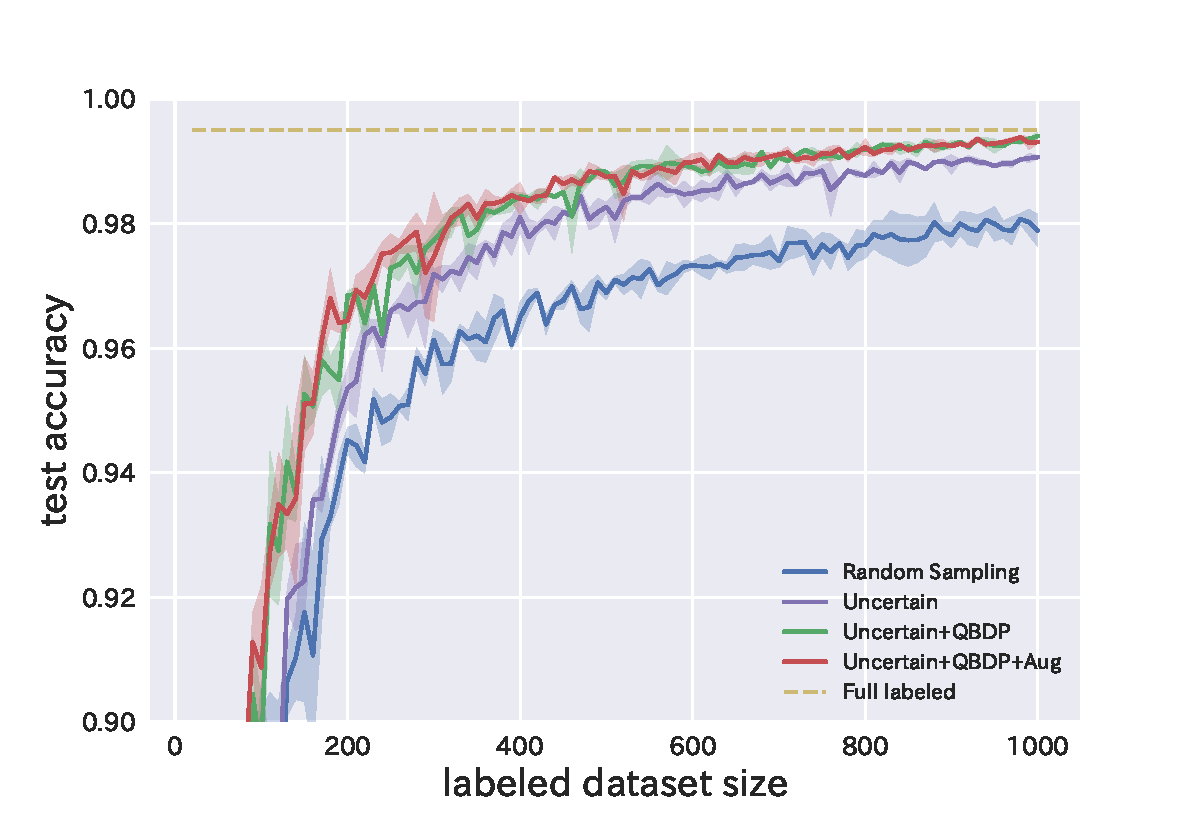
\includegraphics[width=10cm]{figures/mnist_acc_graph.pdf}
     \end{center}
    \caption{各手法を利用した場合のラベル付きサンプル数の増加に対するテスト精度の変化を示した図}
\end{figure}

\begin{table}[b]
    \label{table:mnist_samplenum_accuracy}
    \caption{それぞれのクエリ選考基準を利用した場合にテスト精度を達成するために要したラベルの数}
    \center
    \begin{tabular}{c|c|c|c} 
         & $90\%$ & $95\%$ & $98\%$ \\ \hline
        Random & 110 $\pm$ 20 & 240 $\pm$ 10 & 900 $\pm$ 70 \\
        Uncertain Sampling & 180 $\pm$ 5 & 270 $\pm$ 20  & 600 $\pm$ 50 \\
        Uncertain + QBC + Clustering & 100 $\pm$ 10 & 150 $\pm$ 20 & 320 $\pm$ 10 \\ 
        Uncertain + QBC + Clustering + DA & 90 $\pm$ 0 & 150 $\pm$ 5 & 300 $\pm$ 30 \\

    \end{tabular}
\end{table}

\section{考察}
以下にラベル付きデータセットサイズが100の時にクエリとして選択されたサンプルを示す。図\ref{fig:mnist_query_sample}
QBCがDeepと相性が良いことがわかった。
また、それを示すために訓練データとテストデータに対してDropoutを利用した場合のそれぞれの分布の分散を比較した。
